\documentclass[12pt]{article}
\usepackage{epsf,epic,eepic,eepicemu}
%\documentstyle[epsf,epic,eepic,eepicemu]{article}
\usepackage[cp1250]{inputenc}
\usepackage{graphicx}








\begin{document}
%\oddsidemargin=-5mm \evensidemargin=-5mm \marginparwidth=.08in
%\marginparsep=.01in \marginparpush=5pt \topmargin=-15mm
%\headheight=12pt \headsep=25pt \footheight=12pt \footskip=30pt
%\textheight=25cm \textwidth=17cm \columnsep=2mm \columnseprule=1pt
%\parindent=15pt\parskip=2pt








\begin{center}
\bf Semestral project MIE-PAR 2012/2013:\\[5mm]
    Parallel algorithm for problem\\[5mm]
       Timur\\
       Tatarshaov\\[2mm]
master degree, FIT CVUT, Thakurova 9, 160 00 Praha 6\\[2mm]
\today
\end{center}








\section{Problem definition and description of sequential solution}


\textbf{Problem QUC: queens on chessboard}      
 
       
       \textbf{Task:}


For chessboard S of size n x n, find a placement of the minimal number of queens such that they can attack all chessboard positions and they do not threaten themselves. Queens can attack in all 8 directions, i.e., horizontally, vertically, and diagonally.
       The sequential algorithm is of type SB-DFS with the search depth bounded by n*n. An internal state is defined as a two-dimensional array, which represents the board with placed queens and attacking positions. State considered as a solution if there is no space to place more queens on the board(i.e. all positions in array is marked as taken or attacked).
       Input data are size of the board and placements of starting queens with attacked positions(i.e. two-dimensional array with marked positions).
       Output data is a two-dimensional array with placed queens and attacked positions.
       
       Time measurements of sequential instances for different problem sizes.
       
    Measurements of running time for problems sizes:

1.   Board size 9x9. One queen placed 1055.36s

2.   Board size 10x10. Two queens placed 1152.76s

3.   Board size 7x7. 0 queens placed 139.06s
       









\section{Description of parallel algorithm and its implementation using MPI}









Let's assume this terms:

0-processor, master or main processor(node) -- processor with zero rang which behaves as coordinator among slaves.

Slave processor(node) -- all other processors but 0-processor.

Board -- two dimensional array of integers.

Queen addition -- marking position respected attacking positions on the board.

Free place(position) -- not marked position on the board.

Algorithms starts with following standard MPI commands used.

/* start up MPI */

\verb| MPI_Init |

/* find out process rank */

\verb| MPI_Comm_rank |

/* find out number of processes */

\verb| MPI_Comm_size |

At this step program also retrieves number of processors to use this value for counting when sending tasks to slave nodes.

Algorithm acts in parallel as following.
Main processor starts with input data as a stack with one element which is board probably with queens put on it(depends on input data). It sequentially adds queens to the board on free places, in all possible combinations, for each number of queens.
Marked board pushes to the back of the stack with boards of this combination. On each next step for one more queen addition, algorithms takes board with marked positions from the top of the stack and marks it.
If number of the queens on the board are equal to (floor(SIZE/4) + 1), where SIZE is number of places on the side of the board, main processor sends board to the slave in turn \verb|(MPI_Send).| The it adds rank of that slave, to the arrays of working slaves.
Then main node starts to waiting for data from slave nodes.
After receiving marked boards back from these slaves \verb|(MPI_Recv).| Master compares number of queens on the board with, smallest previously receiving board. And make smallest of them next for comparison.
In result master processor gets board with the smallest number of queens.
And sends signal for stop waiting for data to slaves. Program makes output and then terminates.

Slave nodes behaves similar way, for marking queens. But there is a different communication approach for them. From start they blocked and waiting for the marked board \verb|(MPI_Recv)| for computations. Then slave computes board the way main processor does. After getting full board(without free places) it sends board to the 0-processor \verb|(MPI_Send).|
Besides that slave node waiting(in non-blocking receive)\verb|(MPI_Iprobe)| for data with special tag, which signals that work of slave is finished and there is no need for blocking receive any more. Slave finished his job in that case.

Program finishes execution and does following MPI command at the end.

/* shut down MPI */

\verb| MPI_Finalize|

Size of the board defined as constant in the beginning of the file as SIZE.

To execute application needed following parameters.
pairs of x and y coordinates to put queens there(starting with 0) in following format x y

Execution example
./queens 0 0 2 1




\section{Measured results and evaluation}




\begin{center}
  \begin{tabular}{ | l | c | c | c | c | c | c | c | }
    \hline
    p & 1 & 2 & 4 & 8 & 16 & 24 & 32  \\ \hline
    ps 1 & 1055.36 & 141.92 & 55.06 & 38.51 & 33.35 & 25.43 & 18.81  \\
    ps 2 & 1152.76 & 321.32 & 146.08 & 75.45 & 40.84 & 38.05 & 30.72  \\
    ps 3 & 139.06 & 14.03 & 5.36 & 2.44 & 1.86 & 1.31 & 1.15  \\ \hline
    speedup ps1 & - & 7.44 & 19.17 & 27.40 & 31.64 & 41.50 & 56.11 \\
    speedup ps2 & - & 3.59 & 7.89 & 15.28 & 28.23 & 30.30 & 37.52 \\
    speedup ps3 & - & 9.91 & 25.94 & 56.99 & 74.76 & 106.15 & 120.92 \\
    \hline
  \end{tabular}
\end{center}

Problem set 1 - ps1.   Board size 9x9. One queen placed

Problem set 2 - ps2.   Board size 10x10. Two queens placed 

Problem set 3 - ps3.   Board size 7x7. 0 queens placed 


\clearpage

\textbf{Graphs}
\begin{center}

Problem set 1

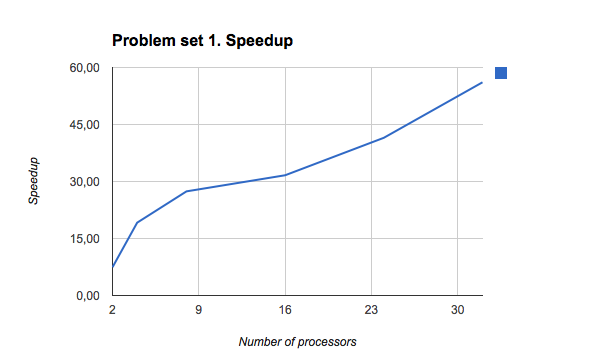
\includegraphics[width=0.9\textwidth]{graphs/ps1.png}

Problem set 2

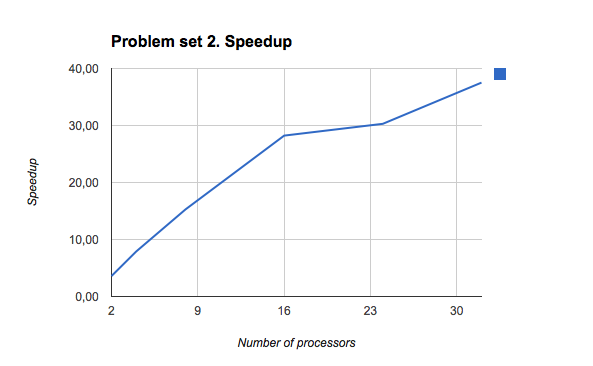
\includegraphics[width=0.9\textwidth]{graphs/ps2.png}

\clearpage

Problem set 3

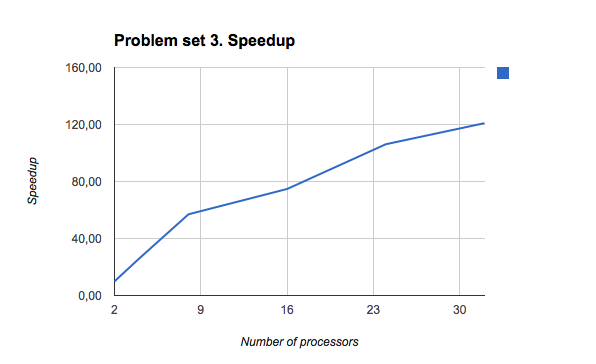
\includegraphics[width=0.9\textwidth]{graphs/ps3.png}

\end{center}




\textbf{Parallel communication subsystem}

Parallel communication subsystem made efficiently but there are still some not probably not critical improvements that can be done.
Firstly main processor waits for results from sub nodes in blocking receive in the same order it sends it. That means that even tasks were send in a possibly equal amount per each node there is a possibility that main processor could wait for some slow slave in the middle results when others will be already finished their jobs. But even while main node have to wait finishing sub computations, some calculations can be done instead of waiting, so communications can be improved in that way, but it wont make dramatical increase possibly.







\section{Conclusion}




Accepting nowadays human needs of huge amounts of data to be processed not comparable with speed of one computer unit requirement in parallel calculations is certain.
In result of making this project, huge valuable experience of new technology has been gotten. Parallel computation requires extra effort of planning communication architecture. And not less of work for building algorithms for parallel work. But if done properly it can dramatically increase speed of processing large amounts of jobs.








\section{Bibliography}

\begin{itemize}

\item Parallel programming, Baker, Lou and Smith, Bradley J 1996
\item Parallel programming with MPI, Pacheco, Peter S 1997

\end{itemize}






\end{document}